%\documentclass{article} %[twocolumn]
\documentclass[AMA,STIX1COL]{WileyNJD-v2}

\articletype{Main paper}%

%\usepackage{algorithmic}
\usepackage{algorithm}
\usepackage{algorithmicx}
\usepackage{algpseudocode}
\usepackage{booktabs}
\usepackage{array}
\usepackage{graphicx}
\usepackage{amsmath}
\usepackage{amsfonts}
\usepackage{amssymb}
\usepackage{multirow}
\usepackage{url}

\received{26 April 2016}
\revised{6 June 2016}
\accepted{6 June 2016}

\begin{document}

\title{A hypothesis test of feasibility for external pilot trials assessing recruitment, follow-up and adherence rates}

\author[CTRU]{Duncan T. Wilson*}
\author[CTRU]{Rebecca E. A. Walwyn}
\author[CTRU]{Julia Brown}
\author[CTRU]{Amanda J. Farrin}

\authormark{Wilson \textsc{et al.}}

\address[CTRU]{Leeds Institute of Clinical Trials Research, University of Leeds, Leeds, UK}

\corres{Duncan T. Wilson, Clinical Trials Research Unit, Leeds Institute of Clinical Trials Research, University of Leeds, Leeds, LS2 9JT.
\email{d.t.wilson@leeds.ac.uk}}

\abstract{
% 250 word limit for SiM
The power of a large clinical trial can be adversely affected by low recruitment, follow-up and adherence rates. External pilot trials estimate these rates and use them, via pre-specified decision rules, to determine if the definitive trial is feasible and should go ahead. There is little methodological research underpinning how these decision rules, or the sample size of the pilot, should be chosen. In this paper we propose a hypothesis test of the feasibility of a definitive trial, to be applied to the external pilot data and used to make progression decisions. We quantify feasibility by the power of the planned trial, as a function of recruitment, follow-up and adherence rates. We use this measure to define hypotheses to test in the pilot, propose a test statistic, and show how the error rates of this test can be calculated for the common scenario of a two-arm parallel group definitive trial with a single normally distributed primary endpoint. We use our method to re-design the TIGA-CUB trial, a pilot trial comparing a psychotherapy with treatment as usual for children with conduct disorders. We then extend our formulation to include estimating the standard deviation of the primary endpoint.
}

% Up to 6 keywords
\keywords{Pilot, external pilot, feasibility, sample size, progression criteria, complex interventions}

\maketitle

\section{Introduction}\label{sec:intro}

Randomised Controlled Trials (RCTs) often fail to recruit to target \cite{Sully2013}, leading to an analysis with less power than intended. Power can also be adversely affected by large rates of attrition, poor adherence to the allocated treatment \cite{Fay2006}, and incorrect specification of a nuisance parameter such as the standard deviation of a continuous endpoint \cite{Teare2014}. A common approach to anticipate these problems is to run a small version of the intended trial, known as an external pilot, to obtain estimates of the relevant parameters and decide if, and how, the definitive trial should be conducted  \cite{Craig2008, Eldridge2016}. This decision is typically made with reference to so-called \emph{Progression Criteria} (PCs), a set of conditions which must be satisfied for the definitive trial to be considered feasible \cite{Avery2017}. In the case of quantitative PCs, parameter estimates are computed using the pilot data and then compared against threshold values. If all estimates exceed their respective thresholds, it is recommended that the definitive trial should be conducted. A recent workshop identified that recruitment, follow-up, and intervention adherence have emerged as common targets of progression criteria \cite{Avery2017}. 

The key role of PCs in pilot trials has led to the CONSORT extension for randomised pilots requiring their reporting \cite{Eldridge2016a}, and the NIHR, one of the major funders of pilot trials in the UK, requiring their pre-specification in the research plan \cite{NIHR2017}. There are ethical and economic imperatives to ensuring PCs are appropriate. If they are too lenient, we increase the risk of proceeding to the definitive trial only to discover it is infeasible, fail to answer the scientific question, in the process wasting resources and subjecting patients to research unnecessarily. If they are too strict, we increase the risk of failing to conduct a definitive trial which would in fact have been feasible, in the process withholding a promising intervention from patients. Despite all this, there is little methodological research available to help researchers determine optimal PCs \cite{Avery2017}. 

%One suggested solution has been to specify two threshold values corresponding to hard `stop' and `go' decisions for each PC \cite{Avery2017}. If an estimate falls between these thresholds an intermediate `modify' decision is suggested, providing the flexibility to argue that the definitive trial will in fact be feasible providing some modifications are made to the intervention or the trial protocol in response to what was observed in the pilot.

%The increasing use of pilot trials has led to several clarifications regarding their definition, design and conduct \cite{Lancaster2004, Craig2008, Arain2010, Thabane2010, Eldridge2016}; an extension to the CONSORT statement \cite{Eldridge2016a}; and a dedicated journal \cite{Lancaster2015}. Despite this, there is little methodological research available to help researchers choose appropriate progression criteria \cite{Avery2017}. 

Another important aspect of external pilot trial design is the choice of sample size. Here, methods have generally focussed on obtaining a sufficiently precise estimate of the standard deviation of a continuous primary outcome to inform the sample size calculation of the definitive trial \cite{Teare2014, Browne1995, Julious2005, Sim2012, Eldridge2015, Whitehead2015}. These methods, often reduced to simple rules-of-thumb such as requiring 35 participants in each arm \cite{Teare2014}, are nevertheless widely used to choose pilot sample size when the estimation of the standard deviation is not the only, or primary, objective. When the goal of the pilot is to provide estimates of recruitment, follow-up and adherence rates and use these in PCs, imprecise estimates will be more likely to meet or miss a PC threshold by chance alone \cite{Eldridge2015, Cooper2018} and thus lead to incorrect progression decisions. This issue will be compounded whenever there are several PCs, with progression to the definitive trial permitted only if all are satisfied. As the number of PCs grows, so does the probability of missing at least one threshold through bad luck, even when the precision around each individual estimate appears adequate - the so-called `reverse-multiplicity' problem seen in multiple testing procedures \cite{Senn2007, Chuang-Stein2007}. Although the sample size of pilots is often justified by reporting the anticipated precision in the estimates of feasibility parameters (e.g. the widths of confidence intervals), there is no clear guidance on how precise they should be, or how to weigh precision against the cost of sampling.


%By choosing both the pilot sample size and the progression criteria without a formal analysis of their resulting statistical properties we risk designing pilots which are unlikely to lead to a `go' decision even when there are no underlying problems; or conversely, unlikely to identify truly infeasible situations before proceeding to the definitive trial.

% As a way to design, we have power or precision arguments. Precision is common in practice, although no guidance as to how to choose n - we use a rule of thumb, then show the CI widthc we would expect, and use that as a justification for n (ref Julious, justification needed but not necesarily a calculation?). So the shortcoming of precision argument is - how precisise is enough? Power does the next step, connecting the precision of estimates to the propoerties of the stop go decision that will be made based on them. So particularly appropriate for early phase studies, where this decision is very explicit and will be made. Note that (PC aside) we will likely have some implicit decision rule in mind, involving comparing CI limits with null and alternative values. But these are equivalent to a test formulation - again, Cocks method is presented in CIs, but can be more explicitly formulated as a test.

A more formal approach to the design and analysis of external pilot trials could employ a hypothesis testing framework. Taking this view, progression to the definitive trial would be determined by comparing an appropriate statistic to a critical value rather than using several independent PCs. To implement this approach we must be able to  identify levels of recruitment, follow-up and adherence which would correspond to feasible or infeasible definitive trials, and identify an approproiate statistic that can differentiate between them. Given these, the critical value and the pilot sample size can then be chosen with regards to the long-run error rates they lead to. %That is, we aim to find a choice of pilot sample size and decision rule such that if the definitive trial is truly feasible we will be unlikely to conclude otherwise (a type II error); and similarly, if the trial is infeasible we will rarely proceed to it (a type I error). 
Although many authors have advised against conducting formal hypothesis tests in pilot trials \cite{Lancaster2004, Arain2010, Thabane2010, Eldridge2015}, these warnings have been in the context of tests of effectiveness. Assuming the effect size of interest is the same in the pilot and the definitive trial and that conventional type I error rates are used, such a test will have low power. Tests assessing rates of recruitment, follow-up and adherence will not necessarily suffer from the same restriction. Moreover, it should be emphasised that the conventional method of pre-specifying several PCs and using these to map pilot data to progression decisions is mathematically equivalent to a multivariate hypothesis test, but without hypotheses being defined and therefore without any understanding of the statistical properties of the resulting procedure. A formal approach is therefore of interest, both to gain an understanding of current practice and to investigate if, and how, progression decisions can be improved. %, which allows an informed choice of both sample size and progression criteria based on the error rates they produce. 

%Despite hypothesis testing being the standard method for the design and analysis of early phase trials in the drug setting (known as `phase II' trials), it is rarely used in pilot trials \cite{Eldridge2016a}. Although some authors have suggested tests of efficacy \cite{Cocks2013, Lee2014}, others have argued such tests will have low power and should be avoided \cite{Lancaster2004, Arain2010, Thabane2010, Eldridge2015}. We are not aware of any methods which use a \emph{formal} hypothesis testing framework to make progression decisions based on feasibility endpoints, although it should be emphasised that the conventional method of pre-specifying PCs and using these to map pilot data to progression decisions is mathematically equivalent to a multivariate hypothesis test, but without hypotheses being defined and therefore without any understanding of the statistical properties (e.g. long-run error rates) of the resulting procedure. 

%Other approaches to testing include methods which explicitly allow for trade-offs between different parameters to be acknowledged \cite{Conaway1996, Thall2008}, a feature commonly seen in pilot trials \cite{Wilson2015}.

The remainder of the paper is structured as follows. First, we will define the specific problem under consideration in Section \ref{sec:problem}. In Section \ref{sec:methods} we will describe a formal hypothesis test of feasibility based on recruitment, follow-up and adherence rates. We will show how null and alternative hypotheses can be defined in terms of the power which will be obtained in the definitive trial, define an appropriate test statistic, and use the statistic's sampling distribution to define and calculate type I and II error rates. We then use the method to re-design an external pilot trial comparing a psychotherapy with treatment as usual for children with conduct disorders in Section \ref{sec:example}. In Section \ref{sec:eval} we study the properties of the proposed test in a range of scenarios and compare its performance against the conventional approach to choosing pilot sample size and PCs. We extend the method in Section \ref{sec:extension} to allow for the additional goal of estimating the standard deviation of the primary outcome, before concluding with a discussion of implications and limitations in Section \ref{sec:discussion}.

% Make the connection with the phase II literature explicit. Testing is standard there as a way to design and analyse, although almost always on efficacy only. General methods for two endpoints have been proposed and are used a lot for efficacy and toxicity, but they have clear shortcomings for us (not lease that we have three endpoints, and particularly the reverse multiplicity problem and inoring trade-offs). What else can we take? Common to relax type I error to maintain a small phase II sample. Connect back to pilot literature where this has also been proposed explicitly \cite{Lee2014}, and implicitly in~\cite{Cocks2013} whose argument is presented in terms of confidence intervals, but is equivalent to powering for a test with 0.5 alpha.

% Shout here that we are considering a frequentist approach

\section{Problem and notation}\label{sec:problem}


Consider an external pilot planned in advance of a large two-arm parallel group trial which will compare an intervention with control based on a normally distributed primary endpoint. We assume that the definitive trial has a target sample size $n_t$ to be recruited from a pool of $n_e$ eligible patients. Each of the $n_e$ eligible patients will agree to take part in the trial with probability $\phi_r$, and recruitment will continue until either the target $n_t$ has been reached or the pool of eligible patients has been exhausted. We denote by $N$ the total number of participants in the definitive trial, a random variable with a truncated binomial distribution of size $n_e$, probability $\phi_r$, and constrained to be less than or equal to $n_t$.

We assume that the $N$ recruited participants of the definitive trial will be randomised equally between the two arms. In the control arm, $F_0$ participants will be successfully followed up with probability $\phi_f$. Thus, $F_0 ~|~ N \sim Bin(N/2, \phi_f)$. In the intervention arm, participants may or may not be followed-up, and may or may not adhere to the intervention. We allow for the possibility that these binary outcomes will be correlated at the participant level by using a multinomial distribution, such that participants will both adhere and be followed up with probability $p_{11}$; adhere, but be lost to follow up with probability $p_{10}$; not adhere, but be successfully followed up with probability $p_{01}$; and neither adhere nor be followed up with probability $p_{00}$. We can parametrise the model with marginal rate of follow-up $\phi_f$, conditional rate of adherence conditional on follow up $\phi_a$, and an odds ratio $\phi_{or}$:
\begin{align*}
p_{11} &= \phi_a \phi_f \\
p_{01} &= \phi_f - p_{11} \\
p_{00} &= \frac{\phi_{or} ~ p_{01}(1-p_{11}-p_{01})}{p_{11} + \phi_{or} ~ p_{01}} \\
p_{10} &= 1 - p_{11} - p_{01} - p_{00}.
\end{align*}
Note that we have assumed a constant marginal rate of follow-up in the intervention and control arms. We denote the number followed-up in the intervention arm by $F_1$, where $F_1 ~|~ N\sim Bin(N/2, \phi_f)$, and the number of those followed-up who also adhere by $A$, where $A ~|~ F_1 \sim Bin(F_1, \phi_a)$. 

We assume that non-adherence will be absolute in the sense that no treatment effect will be gained. We model the outcome for patient $i$ in arm $j$ as
$$
y_{i,j} = t_j a_{i,j} \mu + e_{i,j},
$$
where $t_i$ and $a_{i,j}$ are binary indicators of treatment arm and adherence respectively, $\mu$ is the difference in mean outcome between the two groups, $e_{i,j} \sim N(0, \sigma^2)$ is the residual term, and we have omitted the usual constant intercept for notational simplicity and without loss of generality. We will assume initially that $\sigma^2$ is known, although this will be relaxed in Section \ref{sec:extension}. Also, for the simplicity the primary analysis of the definitive trial will be a complete-case intention-to-treat $z$-test of the observed mean difference $\bar{Y}_1 - \bar{Y}_0$ with a null hypothesis of $H_0: \mu = 0$, where $\bar{Y}_j = \frac{1}{F_j} \sum_{i=1}^{F_j} y_{i,j}$.

We assume that the external pilot trial will take the same form as the definitive trial, but on a smaller scale. The model of recruitment, follow-up and adherence in the pilot trial is assumed to be the same as for the definitive trial apart from one aspect: for the small external pilot trial we will continue recruiting until the target pilot sample size of $n_p$ has been reached. Thus, we consider the achieved sample size of the pilot to be known and fixed, with the number of eligible patients approached but declining to participate following a negative binomial distribution $S \sim NB(n_p, \phi_r)$. Denoting the parameters by $\phi = (\phi_r, \phi_f, \phi_a)$, the external pilot trial will provide an estimate $\hat{\phi}$. In what follows we show how a decision rule mapping $\hat{\phi}$ to the set $\{stop, go\}$ of progression decisions can be defined, and how the parameters of the rule and the pilot sample size $n_p$ can be chosen to obtain an appropriate balance of type I and II error rates and the cost of sampling in the pilot.

\section{A hypothesis test of feasibility}\label{sec:methods}

%In this section we will describe the relevant power function $g(\phi)$, a statistic $s(\hat{\phi})$ and its sampling distribution in the pilot, and a way to calculate the error rates resulting from specific choices of pilot sample size $n_p$ and critical value $c$.

\subsection{Power of the definitive trial}\label{sec:power}

The power of the definitive trial is determined by the sampling distribution of the difference in group means, $\bar{Y}_1 - \bar{Y}_0$. We assume that the definitive trial per-arm sample size will be greater than 30, allowing the sampling distributions of the group means to be approximated by normal distributions. The power of the definitive trial to detect a difference $\mu$ is then
$$
\Phi \left(\frac{\mathbb{E}[\bar{Y}_1 - \bar{Y}_0 ~|~ \mu]}{\sqrt{Var(\bar{Y}_1 - \bar{Y}_0 ~|~ \mu)}} - z_{1-\alpha} \right),
$$
where $\alpha$ denotes the (one-sided) type I error rate. The expectation and variance of the mean difference will depend on the values of $\mu, \phi, n_t$ and $n_e$. For clarity, we will drop the terms $\mu, n_t$ and $n_e$ from our notation as they can be considered fixed. Focussing on power as a function of $\phi$, we use the notation
$$
g(\phi) = \Phi \left( x(\phi) - z_{1-\alpha} \right).
$$
The appendix will show that
$$
x(\phi) =  \frac{ \phi_a\mu \sqrt{\phi_f \mathbb{E}[N ~|~ \phi_r]} } {\sqrt{4\sigma^2 + 2 \mu^2 \phi_a(1-\phi_a)}},
$$
where $\mathbb{E}[N ~|~ \phi_r]$ is the expected number of participants recruited into the definitive trial,
$$
\mathbb{E}[N ~|~ \phi_r] = \sum_{k=0}^{n_t-1} k{n_e \choose k} \phi_r^k (1-\phi_r)^{n_e - k} + n Pr(C \geq n_t),
$$
and $C \sim Bin(n_e, \phi_r)$.

\subsection{Hypotheses and test statistic}

We propose to define points in the null and alternative hypotheses by considering the power which would be obtained in the definitive trial for some $n_t, n_e$. Specifically, we choose $p_0$ so that, for a definitive trial aiming to recruit $n_t$ participants out of a pool of $n_e$ eligible patients, if the power of the trial was known to be less than or equal to $p_0$ then it would be considered infeasible and we would like to minimise the chance of mistakenly proceeding to the definitive trial (a type I error). Similarly, $p_1$ should be chosen so that a definitive trial with power at least $p_1$ and of size $n, n_e$ would be considered feasible and we would like to minimise the chance of mistakenly concluding otherwise and discarding an otherwise promising intervention (a type II error). We can then define null and alternative hypotheses respectively by
\begin{align*}
\Phi_0 &= \{\phi \in \Phi ~ | ~ x(\phi) \leq x_0 \} \\
\Phi_1 &= \{\phi \in \Phi ~ | ~ x(\phi) \geq x_1 \},
\end{align*}
where
$$
x_i = \Phi^{-1}(p_i) + z_{1-\alpha}.
$$

Testing feasibility in the external pilot trial will involve calculating a statistic based on the pilot estimate $\hat{\phi}$ and proceeding to the definitive trial if and only if it exceeds some pre-specified  critical value $c$. A natural choice of statistic is $x(\hat{\phi})$. We can then define the type I and II error rates of the pilot trial:
\begin{align}\label{eqn:ocs}
\alpha = \max_{\phi \in \Phi_0} Pr[ x(\hat{\phi}) > c ~ | ~ \phi, n_p], \\
\beta = \max_{\phi \in \Phi_1} Pr[ x(\hat{\phi}) < c ~ | ~ \phi, n_p].
\end{align}

%\begin{table}
%\centering
%\caption{Notation.}
%\begin{tabular}{l p{8cm}}
%\toprule
%$\phi_r$ & Recruitment rate \\
%$\phi_a$ & Adherence rate \\
%$\phi_f$ & Follow-up rate \\
%$\phi$ & $(\phi_r, \phi_a, \phi_f)$ \\
%$n_e$ & number of eligible participants expected to be approach for consent \\
%$n_t$ & target sample size (per arm) of the definitive trial \\
%$\mu$ & Between group difference \\
%$t_i$ & Binary treatment arm indicator for participant $i$ \\
%$a_i$ & Binary treatment adherence indicator for participant $i$ \\
%$\bar{Y}_j$ & Mean response in arm $j$ \\
%$C$ & Number of consenting participants (per arm) \\
%$R$ & Number of successfully recruited participants (per arm) \\
%$F_j$ & Number of participants successfully followed-up in arm $j$ \\
%$A$ & Number of participants who adhere to treatment in the intervention arm \\
%$g(\phi)$ & Power of the definitive trial conditional on $\phi$ \\
%$R_p^-$ & Number of eligible participants who do not consent to the pilot trial \\
%$h(n_p, c, \phi)$ & Power of the pilot trial with $n_p$ participants in each arm, critical value $c$, and conditional on $\phi$ \\
%\bottomrule
%\end{tabular}
%\end{table}

\subsection{Power of the external pilot trial}

Denote by $n_{af}$ the value taken of the multinomial variable recording follow-up and adherence outcomes, and by $\mathcal{N}_{af}$ the set of possible realisations. The power of the pilot trial can be calculated by considering each possible realisation of recruitment, follow-up and adherence outcomes, calculating the statistic and comparing with critical value $c$, and then summing the indicators of test success weighted by the probabilities of the corresponding pilot data. Formally, the power of a pilot with $n_p$ participants in each arm, critical value $c$, and true parameter values $\phi$, is approximately
\begin{align}\label{eqn:pilot_pow}
h(n_p, c, \phi) &= \sum_{n_{af} \in \mathcal{N}_{af}} \left( \sum_{s = 0}^{s_{max}} 
I \left[ x(\hat{\phi}) > c \mid  s, n_{af}, \phi \right] p_{s}(s | \phi) \right)     
p_{af}(n_{af} |\phi).
\end{align}
Here, $p_{af}(.)$ is the multinomial density describing follow-up and adherence outcomes, and $p_{s}(.)$ is the negative binomial density describing recruitment. The approximation comes from the inner summation term over the number of eligible participants who do not consent being limited to a finite $s_{max}$. We set  $s_{max}$ to the upper 0.999 quantile of the negative binomial distribution, ensuring an accurate approximation whilst avoiding excessive computation.

Equation \ref{eqn:pilot_pow} allows for follow-up and adherence outcomes to be correlated, which may be appropriate if we expect that a participant who does not adhere to the intervention delivery is also less likely to adhere to other aspects of the trial protocol, including data collection. If this is not thought to be the case, we can assume follow-up and adherence are independent and equation \ref{eqn:pilot_pow} simplifies to
\begin{equation*}
h(n_p, c, \phi) = \sum_{a=0}^{n_p} \left[  \sum_{f=0}^{2n_p} \left( \sum_{s = 0}^{s_{max}} 
I \left[ x(\hat{\phi}) > c \mid  s, f, a, \phi \right] p_{s}(s | \phi) \right) p_{f}(f |\phi)  \right] p_a(a | \phi).
\end{equation*}
By avoiding a summation over the multinomial space $\mathcal{N}_{af}$, which can be very large for moderate $n_p$, this reduces the number of terms to be summed and thus decreases computational time. 

%[RW - when would this assumption be reasonable in practice?] [What are the implications? In discussion and in the appendix examples, need to give an indication of how much longer the computations are when we have the more general case]

%Under this model, the power of a pilot trial with $n_p$ participants in each arm, critical value $c$, and true parameter values $\phi$, is
%\begin{align}
%g(n_p, c, \phi) &= \sum_{a = 1}^{n_p} \left( \sum_{f = 1}^{2n_p} 
%Pr \left[ \hat{\phi}_r \hat{\phi}_f \hat{\phi}_a^2 > c \mid f, a, \phi \right]    
%f_f(f | a, \phi) \right) f_a(a | \phi) \\
%&= \sum_{a = 1}^{n_p} \left( \sum_{f = 1}^{2n_p} 
%Pr\left[ \frac{2n_p}{r_{-} + 2n_p} \frac{f}{2n_p} \frac{a^2}{n_p^2} > c \mid f, a, \phi \right]    
%f_f(f | a, \phi) \right) f_a(a | \phi) \\
%&= \sum_{a = 1}^{n_p} \left( \sum_{f = 1}^{2n_p} F_{r_-} \left( \left\lfloor\frac{a^2f}{n_p^2c} \right\rfloor - 2n_p \mid f,a,\phi \right)  f_f(f | \phi) \right) f_a(a | \phi)
%\end{align}

%In the above we assumed that the number of adherers and the number of follow-ups are independent. We might argue that this won't be the case - an individual who sticks to the protocol is more likely to also stick with the trial and give the follow-up data. This won't be any more complicated as we can easily put the joint distribution into the above, but we will have an extra nuisance parameter in the correlation. We can start by assuming this is known. From above we know that we only need 2 out of the 3 necessary parameters of the joint distribution to define our hypotheses. 

\subsection{Operating characteristics}\label{sec:ocs}

Recall that the type I (II) error rate of the pilot trial is defined as the largest probability of proceeding (failing to proceed) to the definitive trial when the true parameter is in the null (alternative) hypothesis. That is, 
\begin{align*}
\alpha(n_p, c) &= \max_{\phi \in \Phi_0} ~ h(n_p, c, \phi) , \\
\beta(n_p, c) &= \max_{\phi \in \Phi_1}  ~ 1 - h(n_p, c, \phi).
\end{align*}
Designing a pilot trial could proceed by considering a set of candidate sample size values $n_p$ and critical values, solving the above optimisation problems for each, and then choosing the $(n_p, c)$ pair which is deemed to give the best balance between the costs of sampling and the two types of errors. This approach has the drawbacks of requiring an appropriate range of $c$ \emph{a priori}, and a lack of sharing information between the discrete optimisation problems. An alternative formulation which avoids these drawbacks is to (for fixed $n_p$) cast the problem as one of constrained bi-objective optimisation over the space $\mathbb{R} \times \Phi \times \Phi$, simultaneously searching for a critical value $c$ and two points in the parameters space, $\phi_0$ and $\phi_1$, which maximise type I and II error rates whilst satisfying the constraints that $\phi_0 \in \Phi_0$ and $\phi_1 \in \Phi_1$. Formally, we solve

\begin{alignat}{1}\label{eqn:MO_opt}
\max ~ & \left( h(n_p, c, \phi_0) , ~ 1 - h(n_p, c, \phi_1)  \right) \\
\text{subject to} ~ & c \in \mathbb{R}, \nonumber \\ 
& \phi_0 \in \Phi_0, \nonumber  \\
& \phi_1 \in \Phi_1. \nonumber 
\end{alignat}

A problem of this nature can be solved numerically using the NSGA-II algorithm \cite{Deb2002}, as implemented in the R package `mco' \cite{Mersmann2014}. It will provide a set of critical values and corresponding points in the null and alternative hypotheses offering different balances between type I and type II error rates. These error rates can then be plotted for a number of choices of $n_p$, and an appropriate design selected from them.

\subsection{Comparison}

An alternative to the proposed test is to follow the conventional approach and make the stop/go decision based on several independent progression criteria. Decision rules are then defined by three critical values $\mathbf{c} = (c_f, c_a, c_r)$, where we proceed to the definitive trial only when $\hat{\phi}_f > c_f$, $\hat{\phi}_a > c_a$ and $\hat{\phi}_r > c_r$. Assuming independence between the parameter estimates, the probability of this event is
\begin{align*}
f(n_p, \mathbf{c}, \phi) &= Pr[\hat{\phi}_r > c_r ~ | ~ \phi] \times Pr[ \hat{\phi}_f > c_f ~ | ~ \phi] \times Pr[ \hat{\phi}_a > c_a ~ | ~ \phi] \\
&= F_s( 2n_p/c_r - 2n_p ~ | ~ \phi) \times [1-F_f(2n_p c_f ~ | ~ \phi)] \times [1-F_a(n_p c_a ~ | ~ \phi)],
\end{align*}
where $F_s(.), F_f(.)$ and $F_a(.)$ are the cumulative distribution functions for the random variables $S, F$ and $A$ in the pilot, respectively. For any given choice of pilot sample size $n_p$ and progression criteria $\mathbf{c}$, type I (II) error rates are defined as before by maximising $f(n_p, \mathbf{c}, \phi)$ over the null (alternative) hypotheses. To find a set of progression criteria which offer different trade-offs between minimising type I and II error rates, we solve the following bi-objective optimisation problem:

\begin{alignat*}{1}
\min_{\mathbf{c} \in [0,1]^3} ~ & \left( \max_{\phi \in \Phi_0} f(n_p, \mathbf{c}, \phi) , ~ \min_{\phi \in \Phi_1} f(n_p, \mathbf{c}, \phi) \right). \\
\end{alignat*}

We use NSGA-II again to solve the outer bi-objective minimisation problem, and the base R `optim' function for the inner optimisations.

\section{Application to an external pilot trial of a psychotherapy intervention}\label{sec:example}

TIGA-CUB was a two-arm, parallel group, individually-randomised external pilot trial aiming to determine the feasibility of a definitive trial comparing second-line, short-term, manualised psychoanalytic child psychotherapy with treatment as usual for children with conduct disorders. The trial's objectives included estimation of the rate at which eligible dyads (where a child - carer dyad was the unit of randomisation and observation) consented to take part in the trial; the level of missing data in the primary outcome; the rate of adherence to the intervention; and the parameters required for the sample size calculation of the main study. Progression criteria relating to recruitment, follow-up and adherence rate were specified, with the definitive trial to go ahead only if:
\begin{enumerate}
\item Recruitment was to target;
\item Attendance was at more than 50\% of sessions in the intervention arm;
\item At least 75\% of follow-up data was collected.
\end{enumerate}

The sample size was determined by using the rule-of-thumb that 30 participants per arm is sufficient to estimate a standard deviation of a continuous primary outcome which is common across arms \cite{Lancaster2004}. Assuming 90\% of pilot participants are followed-up, a sample size of 60 participants in total was chosen and justified in terms of the expected width of 95\% confidence intervals around estimates of the standard deviation (0.39 multiplied by SD), the follow-up rate ($\pm 7$\%), and the adherence rate (between $\pm 8$\% to 18\%).

To apply the proposed method, we assumed a common primary outcome standard deviation of $\sigma = 1$ and an effect size of $\mu = 0.3$ to be detected in the definitive trial. Noting that a total sample size of  $468$ would give a power of 90\% under perfect follow-up and adherence, we set the definitive trial target sample size to $n_t = 515$ to allow for 10\% loss to follow-up. For illustration, we assumed a pool of $n_e = 1000$ eligible participants would be available to recruit from. For the pilot hypotheses, we considered that a definitive trial achieving 80\% power would be of interest, while a power of 65\% or less would be considered infeasible and to be avoided. Thus, $p_1 = 0.8$ and $p_0 = 0.65$. The boundaries of the resulting hypotheses $\Phi_0$ and $\Phi_1$ are plotted in Figure \ref{fig:hyps}. The trade-offs between the three parameters are clear, with decreases in one being compensated by increases in the others in order to maintain power. As the recruitment rate increases beyond around 0.5 there are no opportunities for trade-offs with the remaining parameters because it becomes certain that the recruitment target of $n_t$ will be met, and so the sample size will not increase.

%RW - comment on null versus alternative?

\begin{figure}
\centering
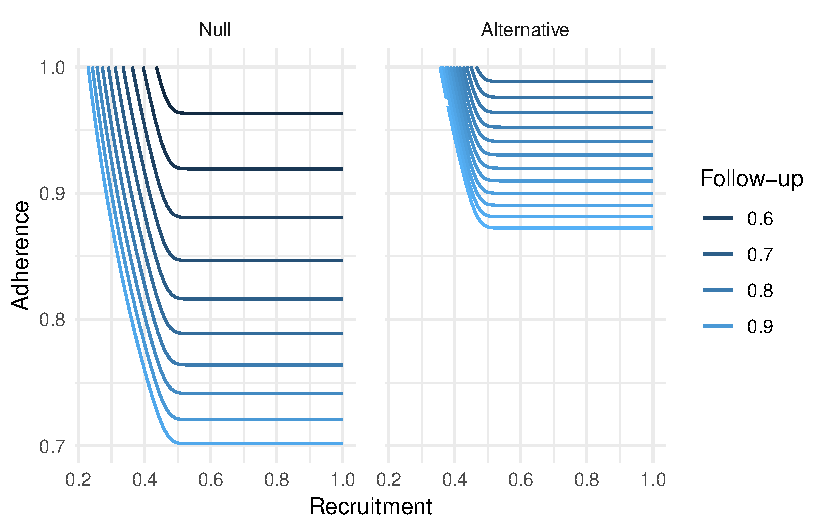
\includegraphics[scale=0.8]{./Figures/hyps.pdf}
\caption{Values of recruitment, follow-up and adherence parameters for leading to a definitive trial power of $p_0 = 0.65$ (i.e. the boundary of the null hypothesis, left panel), or $p_1 = 0.8$ (i.e. the boundary of the alternative hypothesis, right panel).}
\label{fig:hyps}
\end{figure}
% Note - RW asked for line types but can't get these on our continuous binned contour data. Can use direct labels but not clear that the contours are or p_f values
% - also, RW asked for figs after text but note we are using the journal's style file

Given the hypotheses and assuming follow-up and adherence rates are independent, we solved the optimisation problem described in Section \ref{sec:ocs} to obtain operating characteristic curves for external pilot sample sizes of $n_p = 30, 50, 100$ per arm. To provide a comparison with the proposed method, we also calculate the error rates available using the standard approach to setting progression criteria. The results are shown in Figure \ref{fig:ex_ocs}, where we see that operating characteristics for the proposed method and with the original sample size of $n_p = 30$ are quite poor in comparison to the nominal values typically seen in early phase drug trials. For example, a type I error rate of around 0.1 corresponds to a type II error rate of just under 0.4. As we would expect, increasing the external pilot sample size leads to improved error rates. A pilot sample size of 50 participants per arm, for example, reduces the type II error rate to around 0.2 whilst maintaining type I error rate at 0.1.

\begin{figure}
\centering
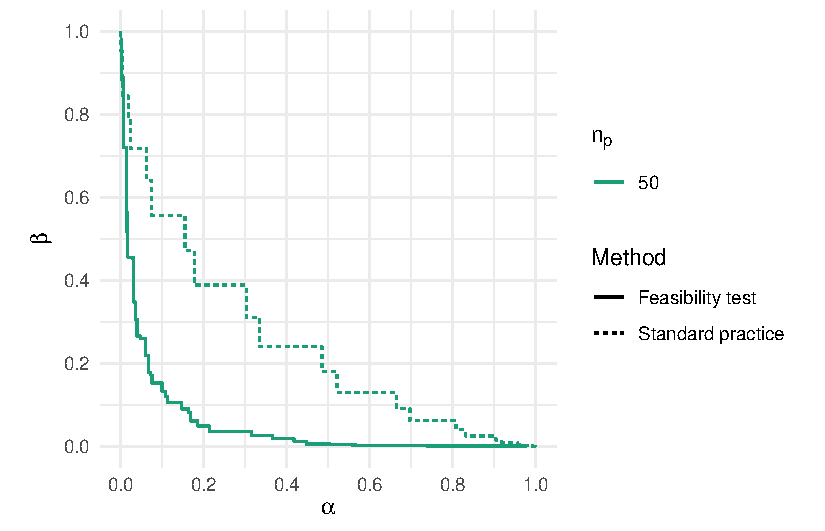
\includegraphics[scale=0.8]{./Figures/ex_ocs.pdf}
\caption{Type I ($\alpha$) and type II ($\beta$) error rates obtained for a range of critical values $c$ and pilot sample sizes $n_p$ when using the proposed method (solid lines). Error rates available when using conventional progression criteria are shown for comparison (dashed lines).}
\label{fig:ex_ocs}
\end{figure}

In terms of the comparator, Figure \ref{fig:ex_ocs} shows that, regardless of the PC thresholds used, the standard procedure of setting several independent PCs is very inefficient in comparison to the proposed test. For example, the operating characteristic curve obtained from a sample size of 100 is slightly worse than that obtained by the proposed test with only 30 participants per arm. The stepped nature of the operating characteristic curves, which becomes more pronounced as the pilot sample size decreases, results from the binary nature of the three endpoints under consideration.

An alternative view results from the observation that if $p_1$ is fixed, we can find a critical value $c$ which will lead to some desired pilot type II error rate independently of $p_0$. Keeping the critical value fixed, we can then look at a range of values for $p_0$ and plot the corresponding type I error rate. For example, taking $p_1 = 0.8$ and asking for a pilot type II error of 0.1, Figure \ref{fig:alt} shows how the type I error rate of the pilot increases with $p_0$ for $n_p = 30, 50, 100$. This shows that, for example, while a large pilot sample of $n_p = 100$ will ensure we will almost never proceed to a definitive trial with a true power of $p_0 = 0.6$, it will also mean that when $p_0 \approx 0.75$ there will only be a 0.5 chance of proceeding. This might be considered rather low, when we have defined the alternative hypothesis using $p_1 = 0.8$. In comparison, the associated values when $n_p = 50$ are around 0.08 and 0.76.

\begin{figure}
\centering
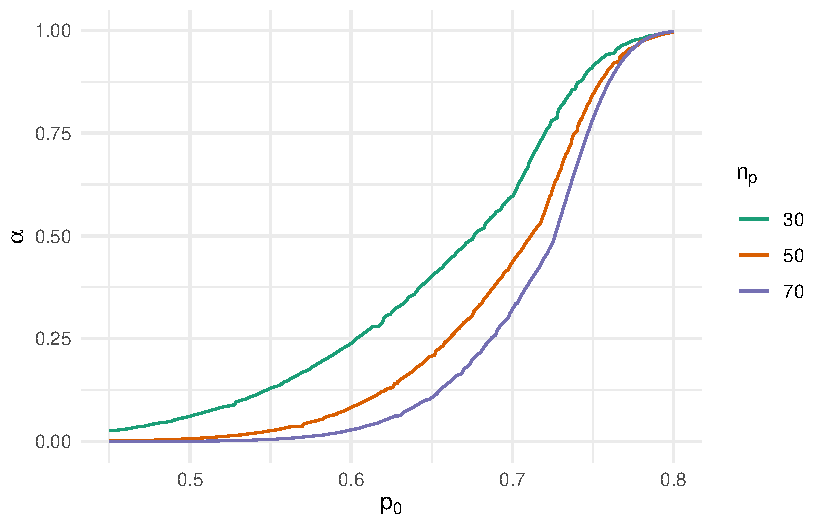
\includegraphics[scale=0.8]{./Figures/alt.pdf}
\caption{Type I error rates for pilot trials of different sample sizes $n_p$, as a function of the null hypothesis parameter $p_0$ and keeping type II error maintained at 0.1.}
\label{fig:alt}
\end{figure}

\section{Evaluation}\label{sec:eval}

To understand the properties of the proposed method more generally, we calculated the error rates available under 9 scenarios with different target sample sizes ($n_t = 468, 514, 562$) and powers defining the null hypothesis ($p_0 = 0.6, 0.65, 0.7$). Throughout, the power defining the alternative hypothesis was kept at $p_1 = 0.8$, the effect size at $\mu = 0.3$, the standard deviation at $\sigma = 1$ and the number of eligible participants at $n_e = 1000$. The target sample sizes were determined by first calculating the number needed to give the definitive trial a power of 90\% under perfect follow-up and adherence, and then inflating this by 10 and 20\% to allow for some anticipated imperfection in these parameters. For each scenario we calculated the operating characteristics of an external pilot with sample size $n_p = 30, 50, 100$ per arm.

%Operating characteristics are not affected by the value of $n_e$ (why? explain), so this was kept constant at 500. They are affected by the standardised effect size to be detected, $\mu/\sigma$, and the target sample size $n_t$, but only through their the power obtained by that sample size for that effect. So, we keep the standardised effect size constant at 0.3, and vary $n_t$.
 
%results
The resulting error rates are illustrated in Figure \ref{fig:eval}. We see that inflating the target sample size leads to a small increase in error rates. For example, for $n_p = 30$, $n_t = 468$ and $p_0 = 0.7$ (top right panel), the pilot can have error rates of $\alpha = 0.094$ and $\beta = 0.557$. Increasing the target sample size to $n_t = 514$ gives an increased type II error rate of $\beta = 0.682$ whilst approximately maintaining type I error, with $\alpha = 0.097$. This general behaviour can be explained by noting that more recruited participants will mean we can tolerate worse follow-up and/or adherence whilst maintaining power, so the hypotheses will expand , and in general we can expect error rates to increase as the size of the hypotheses they are defined over increase. 

% So does this imply we should keep n_t low and never inflate it? Is that what we would have expected? No, these are pilot only - if we didnt inflate in main, we would expect low power?

Error rates are sensitive to the power used to define the null hypothesis. For example, with $n_p = 30$ and $p_0 = 0.7$ one can obtain error rates of $\alpha = 0.094$ and $\beta = 0.557$. If we reduce $p_0$ to 0.6, increasing the distance between the hypotheses, one can reduce type II error to $\beta = 0.14$ in exchange for a negligible increase in type I error to $\alpha = 0.099$. 

The proposed method substantially outperforms the conventional approach in all scenarios, with the latter in some cases proving to be little more effective than tossing a coin as a means of making a stop/go decision (when $p_0 = 0.7$, right column). 

\begin{figure}
\centering
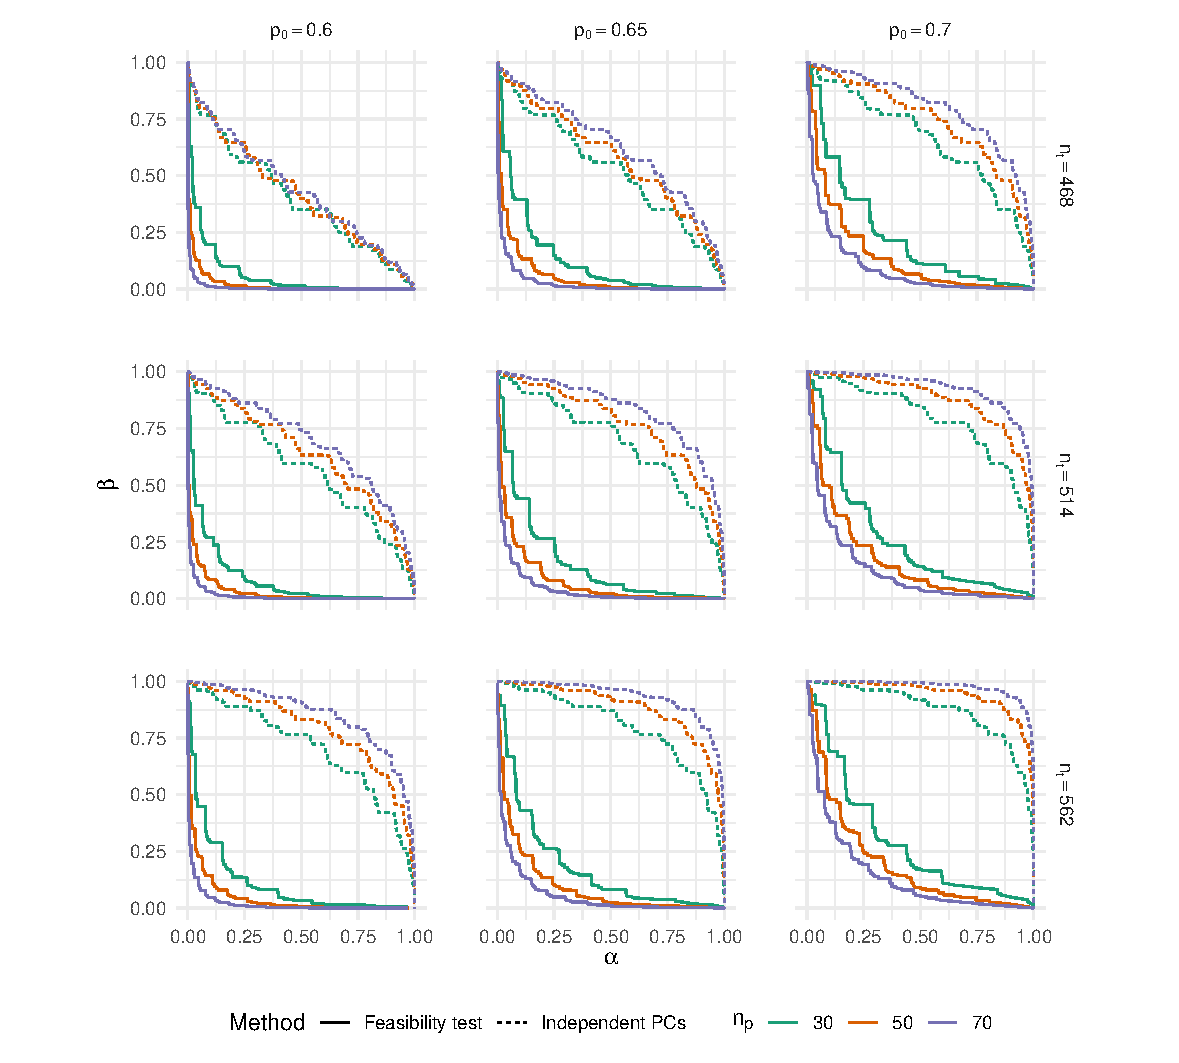
\includegraphics[scale=0.8, trim={1.5cm 0 0 0},clip]{./Figures/eval.pdf}
\caption{Type I ($\alpha$) and type II ($\beta$) error rates obtained for a range of critical values $c$ and pilot sample sizes $n_p$ when using the proposed method (solid lines) and the conventional approach (dashed line). The power used to define the null hypothesis increases from left to right, $p_0 = 0.6, 0,65, 0.7$, while the target sample size of the definitive trial is increased from top to bottom, $n_t = 468, 514, 562$.}
\label{fig:eval}
\end{figure}

\section{Extension - unknown variance}\label{sec:extension}

Thus far we have considered how recruitment, follow-up and adherence rates all affect the power of the definitive trial, and have shown how these can be assessed in an external pilot trial as part of a hypothesis test. Another parameter which affects the power of the definitive trial is the standard deviation of the outcome measure: recall from Section \ref{sec:power} that the conditional power is 
$$
g(\phi, \sigma) = \Phi \left( x(\phi, \sigma) - z_{1-\alpha} \right),
$$
where
$$
x(\phi, \sigma) =  \frac{ \phi_a\mu \sqrt{\phi_f \mathbb{E}[N ~|~ \phi_r]} } {\sqrt{4\sigma^2 + 2 \mu^2 \phi_a(1-\phi_a)}},
$$
We can, therefore, include the true value of $\sigma$ in the definition of the hypotheses $\Phi_0$ and $\Phi_1$, and include the pilot estimate $\hat{\sigma}$ in the test statistic $x(\hat{\phi}, \hat{\sigma})$. This will allow for high variability in the outcome measure, which may lead to a trial with infeasibly low power, to be identified at the pilot stage.

For notational simplicity and ease of computation we will focus on the case where follow-up and adherence are independent, but the method extends naturally to the more general case. The power of the pilot trial is now approximately 
\begin{equation*}
h(n_p, c, \phi, \sigma) = \sum_{a=0}^{n_p} \left[  \sum_{f=0}^{2n_p} \left( \sum_{s = 0}^{s_{max}} 
\left[ \int_0^y p_{\hat{\sigma}^2}( \hat{\sigma}^2 | s, a, f, \phi) ~ d\hat{\sigma}^2 \right] 
p_s(s | \phi) \right) p_{f}(f |\phi)  \right] p_a(a | \phi),
\end{equation*}
where $p_{\sigma^2}(.)$ in the density function of the sample variance, specifically,
$$
\hat{\sigma}^2 ~|~  f \sim \frac{\sigma^2 \chi^2_{f - 1}}{f - 1}.
$$
The upper limit of the integral is
$$
y = \frac{\hat{\phi}_a^2 \mu^2 \hat{\phi}_f \mathbb{E}[N ~|~ \hat{\phi_r}]}{4c^2} - \frac{1}{2} \mu^2 \hat{\phi}_a (1-\hat{\phi}_a).
$$

Empirically, we find that both type I and II error rates increase as the standard deviation decreases. To avoid the trivial situation where error rates tend to 1 as $\sigma$ tends to zero, we include a lower limit on $\sigma_*$ in the definitions of the hypotheses $\Phi_0$ and $\Phi_1$, giving
\begin{align*}
\Phi_0 &= \{\phi \in \Phi, \sigma > \sigma_*  ~ | ~ g(\phi, \sigma) <= p_0 \}; \\
\Phi_1 &= \{\phi \in \Phi, \sigma > \sigma_* ~ | ~ g(\phi, \sigma) >= p_1 \}.
\end{align*}

To illustrate the effect of allowing for uncertainty in $\sigma$, we calculated the error rates available when $n_p = 30, n_t = 514, p_0 = 0.65$ and $p_1 = 0.8$, and the lower limit was taken to be $\sigma_* = 0.8$. We can then compare these error rates with those previously obtained when it was assumed that $\sigma = 1$. Figure \ref{fig:unknown_var} illustrates the impact of relaxing the assumption. For example, recall that when $\sigma$ was assumed known, a pilot trial type I error rate of around 0.1 allowed a type II error rate of around 0.14. Maintaining the same type I error but now estimating $\sigma$ in the pilot increases type II error to 0.51. The detriment stems from two issues. Firstly, by using the pilot estimate in the test statistic $x(\hat{\phi}, \hat{\sigma})$ its sampling variability increases. Secondly, by allowing for the lower limit of $\sigma_* = 0.8$ we accommodate lower values of the rates $\phi_r, \phi_a$ and $\phi_f$ in our hypotheses in much the same way as in Section \ref{sec:eval} when we increased $n_t$, with the same effect of enlarging the hypotheses and thus allowing more extreme error rates to be located. Note that by including a continuous term $\hat{\sigma}$ in our test statistic, we now have a smooth rather than stepped operating characteristic curve.

\begin{figure}
\centering
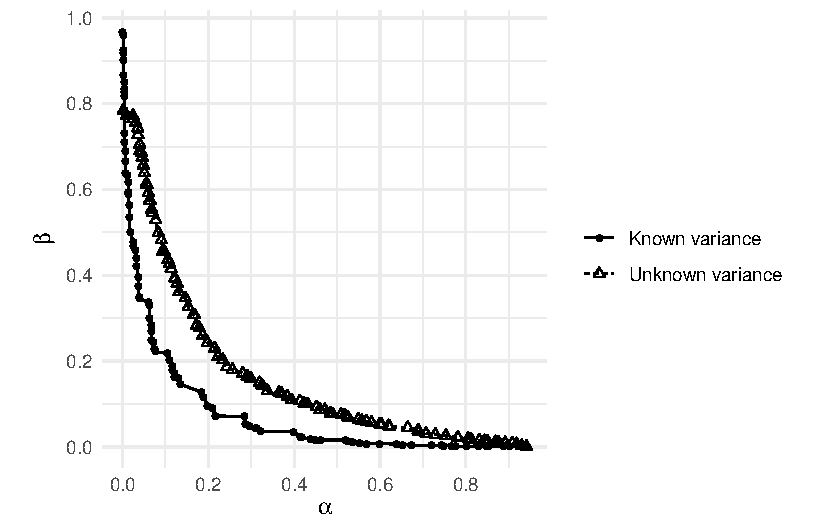
\includegraphics[scale=0.8]{./Figures/var_ocs.pdf}
\caption{Type I ($\alpha$) and type II ($\beta$) error rates obtained for a range of critical values $c$ and pilot sample size $n_p = 50$ when the standard deviation of the primary outcome is either assumed known or estimated in the pilot trial.}
\label{fig:unknown_var}
\end{figure}

\section{Discussion}\label{sec:discussion}

% To add 
% - possible extension to internal pilots
% - assumption of non-differential attrition (can extend easily in theory, but will have another dimension to the search space [so expect more extreme points and worse OCs], and the power calc for the pilot will have another summation over the top so everything will take longer [note that extending the C++ code won't be easy for others, so should we just do it and report how much longer things take?])
% - assumption of absolutre adherence, argue this is conservative [only comes through main trial power] and a more detailed model would be unrealistic prior to a pilot.
% - assumption of primary analysis being complete case ITT z-test - RW says reasonable if simple randomisation used?
% - assumption of fixed pilot trial n, i.e. will not fail to recruit target. Fits in with standard approach to calculating OCs, always assuming a target reached, maybe inflated to allow for extected attrition, with the resulting random sample size not incorporated into design OCs.Pilot stat still fine to use as standardised by actual np, since usuing estimated rates.


We have proposed a statistical test which simultaneously assesses recruitment, follow-up and adherences rates in order to anticipate and mitigate related problems which would render the planned definitive trial infeasible. We have shown that, without increasing the sample size of the pilot trial beyond typical values, the test can limit the probability of mistakenly running an underpowered trial whilst reliably ensuring well-powered trials will progress. Moreover, we have shown the proposed method to be a substantial improvement on the conventional approach to setting progression criteria in pilot trials. We have shown how the test can be extended to include the common pilot objective of estimating an unknown standard deviation nuisance parameter, and found that for this to be incorporated the sample size of the pilot trial will have to be increased.

%\subsection{Intermediate `amber' decisions}

Our method leads to a binary stop/go decision. Increasingly, progression criteria in pilot trials are incorporating three outcomes, adding an additional intermediate `amber' decision between the `red' stop and `green' go \cite{Avery2017}. The intention is that if the pilot estimate is neither clearly good nor bad, but somewhere between, then it may be possible to make some modifications to the intervention or the trial protocol which would ensure the definitive trial will be feasible. A possible extension to the testing framework outlined could consider defining three hypotheses where the decisions `stop', `modify' or `go' would be optimal. A major difficulty in implementing such an approach arises from the fact that, before observing the pilot trial, it will be hard to know for what parameter values a `modify' decision will be optimal. This follows since the type and effect of modification available will generally not be known prior to the pilot. An example referred to in \cite{Avery2017} is of a trial manager being absent on sick leave for much of the pilot. Once this has been identified we might reasonably expect a large improvement in the recruitment rate in the definitive trial if measures to ensure cover of trial managers are put in place; but it would have been impossible to know, prior to the pilot, that such a modification effect was going to be available. A Bayesian approach may help overcome this challenge, allowing uncertainty in any modification effect to be expressed prior to the pilot \cite{Hampson2017}. Although some methods proposed in the phase II drug trial setting have allowed for three outcomes \cite{Storer1992, Sargent2001, Hong2007}, they are designed to allow for other non-primary endpoints to influence the stop/go decision, not to allow for any modifications.

In practice, the pilot trial could be designed using our method and assuming no modifications will be possible, and, in the event that we wish to make modifications, another pilot could be done to assess the effect of these. This would appear to be in line with the MRC framework for complex intervention development and evaluation \cite{Craig2008}, although we are not aware of any examples where two or more pilots have been done in preparation for a definitive trial. Alternatively, if the modifications are made and we proceed directly to the definitive trial, we should be clear that the error rates associated with the pilot trial as designed will no longer apply. Even in the idealised scenario of knowing exactly what the effect of the modification will be, due to the binary nature of the endpoints being assessed in the pilot, error rates will not remain constant if hypotheses and critical values are shifted by the same amount. 
%For example, consider a very simple example where we test one binary endpoint with parameter $\rho$ and our original null and alternative hypotheses are $\rho_0 = 0.7, \rho_1 = 0.8$ with a decision rule of proceeding if and only if $\hat{\rho} > 0.75$. If we become aware that we can modify the intervention and increase the parameter value by 0.2, we may want to shift the hypotheses to $\rho_0 = 0.5, \rho_1 = 0.6$ and decision rule to $\hat{\rho} > 0.75$. However, for a sample size of 60 being used to estimate $\rho$, this transformation will increase the type I error from 0.20 to 0.22 and type II error from 0.17 to 0.21. 
In the more realistic case where the modification effect is estimated with some error as opposed to known exactly, the error rates will deviate from the original numbers even more. 

%\subsection{Adjusting the definitive trial design after the pilot}

We have assumed that the number of eligible patients $n_e$ and the target sample size $n_t$ for the definitive trial are fixed and known when designing the pilot. In practice, the pilot trial feasibility test may suggest a $go$ decision but, based on the pilot estimates $\hat{\phi}, \hat{\sigma}^2$, we may wish to adjust $n_e$ or $n_t$ (for example, in an attempt to obtain a specific nominal power). Modifying the sampling plan of the definitive trial in this manner is possible, but we must clarify the interpretation of hypotheses and error rates. For example, we may have defined the null hypothesis so that $\phi \in \Phi_0 \Leftrightarrow g(\phi, n_e, n_t) \leq 0.6$ (say), yet we could increase the definitive trial sample size to $n_e', n_t'$ such that $g(\phi, n_e', n_t') > 0.9$. Under our formulation, we would still consider $\phi$ to be in the null, and would want to avoid running a definitive trial with sample size $n_e', n_t'$ and power $g(\phi, n_e', n_t') = 0.9$. This corresponds to a belief that the improvement in power obtained by moving from $n_e, n_t$ to $n_e', n_t'$ is not sufficient to justify the increased cost of sampling. Similarly, any point $\phi \in \Phi_1$ in the alternative hypothesis will be still considered so even after adjusting $n_e, n_t$. If we limit ourselves to the option of increasing the definitive trial sample size after the pilot (a common constraint with sample size re-estimation methods in internal pilots\cite{Friede2006}), we believe such adjustments are compatible with our proposed model.

%\subsection{Extending to other types of trial designs}

We have focussed on a specific problem where the definitive trial will have a randomised two-arm design and has a single, normally distributed primary outcome measure. Our method could be applied directly to any problem with an outcome that can be approximately modelled as normal. For example, a binary endpoint can be incorporated using a normal approximation if the definitive trial sample size is sufficiently large; or a cluster randomised trial could be addressed if the endpoints are all measured at the cluster level. To extend the method to other problems, we would require an expression for the power of the definitive trial (as a function of parameters $\phi$), a statistic to use in the pilot trial, and an expression for the power of the pilot trial using that statistic. When analytic forms of the power functions cannot be found, they can be approximated using simulation \cite{Landau2013} and, in principle, the optimisation problem in Section \ref{sec:ocs} could be solved as before. In practice, evaluating two objectives and two constraints using simulation would be computationally demanding and the NSGA-II algorithm would take an infeasibly long time to converge. Future work could explore how efficient global optimisation algorithms \cite{Jones2001} could be used to solve these problems in a timely manner 

%\subsection{Assessing potential efficacy}

In addition to the recruitment, follow-up and adherence rates and the standard deviation we have considered in this paper, another parameter which would be of interest when deciding to run a definitive trial is the treatment effect $\mu$ \cite{Wilson2015}. We could consider incorporating $\mu$ into our method, including it in our hypotheses definitions and its estimate into the pilot test statistic, but there are at least two methodological challenges in doing so. Firstly, as we increase the effect $\mu$ when defining our hypotheses, we will accommodate worse values of the remaining parameters whilst maintaining power. To avoid trivial cases where, for example, a follow-up rate of $\phi_f = 0.01$ is considered acceptable because the treatment effect is so large, an upper limit on $\mu$ would have to be specified when defining the hypotheses. Because error rates are likely to be maximised at this extreme value, operating characteristics will be highly sensitive to the choice of the limit.

A second issue is that, unlike parameters like follow-up rate, the treatment effect is not of interest only in as much as it effects the power of the definitive trial. For example, two points in the parameter space could lead to the same power, but one may be considered in the null and the other in the alternative because the treatment effect in the latter is so much greater. With two attributes of interest (in this case, power and treatment effect), one potentially useful avenue for future research is the use of Bayesian statistical decision theory. In addition to permitting a utility function which could articulate the preferences and trade-offs between multiple attributes, working in a Bayesian framework would also allow us to focus on plausible regions of the parameter space as opposed to extreme points, thus helping to address the first issue.

%\subsection{Other}

A criticism of the proposed method is the simplicity of the decision rule it suggests. Particularly in the case of pilot trials of complex interventions, we would expect the decision of if and how the definitive trial should be conducted to be informed by many factors beyond the pilot estimates of a handful of parameters, not least qualitative outcomes. However, we believe the method will still provide a useful guide to decision making, and allows for the choice of pilot sample size to be considered more fully. This view is supported by the continued prevalence of N-P hypothesis testing for the design and analysis of all types of clinical trials, where the final decision is rarely made by following the result of the test. The proposed method could benefit from further methodological research. The proposed statistic is not guaranteed to be optimal in any sense (e.g. uniformly most powerful), and so further research could consider alternatives and their properties.

%We have assumed adherence is absolute, in the sense that a participant in the intervention arm who doesn't adhere will receive no treatment effect.

\subsection*{Acknowledgements}
A W-H.

\subsection*{Declaration of conflicting interests}

The Authors declare that there is no conflict of interest.

\subsection*{Funding}

This work was supported by the Medical Research Council [grant number MR/N015444/1].

%\bibliographystyle{unsrt}
\bibliography{C:/Users/meddwilb/Documents/Literature/Databases/DTWrefs}

\appendix
%\section*{Derivations}

Recall that the sample means are
\begin{align*}
\bar{Y}_1 &= \frac{A}{F_1}\mu + \frac{1}{F_1} \sum_{i=1}^{F_1} e_{i,1}, \\
\bar{Y}_0 &= \frac{1}{F_0}\sum_{i=1}^{F_0} e_{i,0},
\end{align*}
where $F_j$ denotes the number of participants in arm $j$ who are followed-up, and $A$ denotes the number of participants in the intervention arm who both adhere \emph{and} are follow-up. These sample means have expectations $\mathbb{E}[\bar{Y}_1 | \phi] = \mathbb{E}[\frac{A}{F_1}\mu | \phi] = \phi_a \mu$ and $\mathbb{E}[\bar{Y}_0 | \phi] = 0$. For the variance of the intervention group mean, we have by the law of total variance that
\begin{equation}\label{eqn:int_group_mean}
Var(\bar{Y}_1) = \mathbb{E}[Var(\bar{Y}_1 | F_1, A)] + 
\mathbb{E}[Var(\mathbb{E}[\bar{Y}_1 | F_1, A] | F_1)] + 
Var(\mathbb{E}[\bar{Y}_1 | F_1]).
\end{equation}
Taking each of these terms in turn:
$$
\mathbb{E}[Var(\bar{Y}_1 | F_1, A)] = \mathbb{E} \left[ \frac{\sigma^2}{F_1} \right] = \frac{2\sigma^2}{\phi_f \mathbb{E}[N]},
$$
where $\mathbb{E}[N]$ is the expected number of participants recruited to the trial and randomised equally between arms. Denoting the number of eligible participants who consent by $C$, then,
$$
\mathbb{E}[N] = \mathbb{E}[N ~|~ C < n_t] Pr(C < n_t) + \mathbb{E}[N ~|~ C \geq n_t] Pr(C \geq n_t).
$$
Note that $C$ follows a binomial distribution with size $n_e$ and probability $\phi_r$. Because recruitment will stop once the target has been reached, $\mathbb{E}[N ~|~ C \geq n_t] = n_t$. We also have
$$
\mathbb{E}[N ~|~ C < n_t] = \frac{\sum_{k=0}^{n_t-1} k{n_e \choose k} \phi_r^k (1-\phi_r)^{n_e - k} } {Pr(C < n_t)},
$$
and so 
$$
\mathbb{E}[N] = \sum_{k=0}^{n_t-1} k{n_e \choose k} \phi_r^k (1-\phi_r)^{n_e - k} + n_t Pr(C \geq n_t).
$$
Returning to equation \ref{eqn:int_group_mean}, the second term is 
\begin{align*}
\mathbb{E} \left[ Var(\mathbb{E}[\bar{Y}_1 | F_1, A] ~|~ F_1) \right] &= \mathbb{E} \left[ Var \left(\frac{A\mu}{F_1} ~|~ F_1 \right) \right] \\
&= \mathbb{E} \left[\frac{\mu^2}{F_1^2} Var(A ~|~ F_1) \right] \\
&= \mathbb{E} \left[ \frac{\mu^2}{F_1^2} F_1 \phi_a (1-\phi_a) \right] \\
&= \frac{2\mu^2}{\phi_f \mathbb{E}[N]} \phi_a (1-\phi_a).
\end{align*}
Finally,
\begin{align*}
Var(\mathbb{E}[\bar{Y}_1 | F_1]) &= Var \left( \mathbb{E} \left[ \frac{A \mu}{F_1} ~|~ F_1 \right] \right) \\
&= Var \left( \mathbb{E} \left[ A ~|~ F_1 \right] \frac{\mu}{F_1} \right) \\
&= Var \left( F_1 \phi_a \frac{\mu}{F_1} \right) \\
&= 0.
\end{align*}
This then gives
$$
Var(\bar{Y}_1) = \frac{2\sigma^2}{\phi_f \mathbb{E}[N]} + \frac{2\mu^2}{\phi_f \mathbb{E}[N]} \phi_a (1-\phi_a).
$$

The variance of the control group sample mean is
\begin{align*}
Var(\bar{Y}_0) &= \mathbb{E}[Var(\bar{Y}_0 | F_0)] + Var(\mathbb{E}[\bar{Y}_0 | F_0]) \\
&= \mathbb{E} \left[ \frac{\sigma^2}{F_0} \right] + 0\\
&= \frac{2\sigma^2}{\phi_f \mathbb{E}[N]}.
\end{align*}

The power of the trial can then be obtained by substituting the expectation and variance of the sample means into the usual formula (which, again, assumes they are normally distributed):
\begin{align*}
g(\phi) &= \Phi \left(\frac{\mathbb{E}[\bar{Y}_1 - \bar{Y}_0]}{\sqrt{Var(\bar{Y}_1 - \bar{Y}_0)}} - z_{1-\alpha} \right) \\
&= \Phi \left( \frac{\phi_a\mu}{\sqrt{ \frac{2\sigma^2}{\phi_f \mathbb{E}[N]} + \frac{2\mu^2}{\phi_f \mathbb{E}[N]} \phi_a (1-\phi_a) + \frac{2\sigma^2}{\phi_f \mathbb{E}[N]}} } - z_{1-\alpha} \right) \\
&= \Phi \left( \frac{ \phi_a\mu \sqrt{\phi_f \mathbb{E}[N]} } {\sqrt{4\sigma^2 + 2\mu^2 \phi_a(1-\phi_a)}} - z_{1-\alpha} \right) \\
&= \Phi \left( x(\phi) - z_{1-\alpha} \right),
\end{align*}




\end{document}
